
\chapter{ \uppercase {Residual Monte Carlo Treatment of the Time Variable}}
\label{sec:time}

In this chapter, we have modified the time-discrete HOLO method to include higher-accuracy MC treatment
of the time variable for the radiation unknowns in the TRT equations. 
A potential application where this accuracy is important is stellar atmosphere calculations. 
The ECMC algorithm
is modified to include the time variable, allowing for residual MC integration of the time
variable. The LO equations are closed in time consistently using a parametric closure
derived from the HO equations. The goal is to improve
efficiency compared to IMC, while improving the accuracy compared to the time-discrete
HOLO algorithm.  It is
noted that no adaptive refinement in time is performed, so maintaining exponential convergence
may not be possible.  However, we still expect the residual MC formulation of the ECMC method
to show improvement in efficiency over standard MC.

In the remainder of this chapter, modifications to the HOLO algorithm to include higher
time accuracy are detailed.
First, the inclusion of the time variable into the ECMC trial
space is given, along with modifications to the HO algorithm.
The process of sampling, tracking, and tallying particle histories in time
can be found in literature\cite{wollaber_review,fnc,wollaber_thesis,cj_thesis}, but
sufficient details are provided in this chapter.  Then, a new temporal closure for the LO
equations is given.  Finally, results for the new algorithm are compared to
IMC and the time-discrete HOLO method for accuracy and statistical efficiency.  

\section{Modifications to the HO Solver}
\label{sec:time_ho}

Inclusion of the time variable $t$ in the trial space used by ECMC allows for no discretization of the
transport operator $\B L$.  The transport operator, applied to the continuous intensity
$I$, becomes
\begin{equation}
    \B LI(x,\mu,t) = \frac{1}{c}\pderiv{I(x,\mu,t)}{t}  + \mu \pderiv{I(x,\mu,t)}{x} + \sigma_t I(x,\mu,t)
\end{equation}
The emission source is still treated with a BE discretization, which is
similar to the approximation made in IMC.  Overall, the accuracy in the time variable will be limited by the BE discretized temperature
terms, particularly in optically thick
regions.  However, accuracy in thin regions can be significantly improved.

With this definition of $\B L$ and the temperature discretization, the ECMC algorithm specified in
Sec.~\ref{sec:ecmc} is applied, without further modification.  However, the residual
source and trial-space representation now include $t$.   Each batch is still estimating the error in the
current projection estimate $\tilde I(x,\mu,t)$, but sampling and tallying of the time
variable are included in the MC inversion of the $\B L$
operator.  

\subsection{Step Doubly-Discontinuous Trial Space in Time}

It is necessary to define a new trial space that includes the time variable to explicitly evaluate the residual.
The time variable trial space has a similar representation to the LDD spatial representation 
in Sec.~\ref{sec:ldd}, but the solution is a constant value over
the interior of the time step. This step, doubly-discontinuous (SDD) trial space is defined as
\begin{equation}\label{eq:time_space}
    \tilde I(x,\mu,t) = \left \{ \begin{array}{cl}
        \tilde I^{n}(x,\mu)  & \quad t = t^n \\ 
        \overline I(x,\mu)  & \quad t \in (t^{n},t^{n+1}) \\               
      \tilde I^{n+1}(x,\mu)   &  \quad        t = t^{n+1}
    \end{array}           \right.
\end{equation}
where we have used $\overline I$ to denote the time-averaged LDFE \emph{projection} in $x$
and $\mu$ of the intensity over the interior of the time step;  the beginning and end of
time step projections are denoted $\tilde I^{n}$ and $\tilde I^{n+1}$, respectively.   An
illustration of $t$ for the SDD trial space, over the $n$-th time step, 
is depicted in Fig.~\ref{fig:dd_time}.    There is a projection error incurred by using the LDFE
projection to represent the intensity between time steps.  However, with sufficient noise
reduction and mesh resolution, this should be an acceptable error compared to potentially large
statistical noise of standard MC.
\begin{figure}[H]
    \centering
    \begin{center}
%        \resizebox{0.4\textwidth}{!}{
        \begin{tikzpicture}[scale=0.882, every node/.style={transform shape}]
            \draw (1.0,4.0) node[fill,circle,inner sep=0pt,minimum
            size=4.2pt] {};
            \draw [->] (1.6,4.25) -- (2.4,4.25) node[anchor=west] {$t$};
            \draw (1.0,0.4) -- (1.0,0.6) node[below, pos=0.4] {$t^{n}$};
            \draw (5.90,0.4) -- (5.90,0.6) node[below, pos=0.4] {$t^{n+1}$};
            \node at (3.6,3.06) {$\overline{I}_{HO}(x,\mu)$};
            \draw [thick] (1.0,0.5) -- (5.9,0.5) node[anchor=north west] {};
            \filldraw[color=black, fill=white] (1,2.450) circle (2.1pt);
            \draw (1.0,2.45) -- (5.90,2.45);
            \filldraw[color=black, fill=white] (5.9,2.450) circle (2.1pt);
            \draw (5.9,1.6) node[black,fill,circle,inner sep=0pt,minimum size=4.2pt] {};
            \node[anchor=west] at (5.9,1.6) {${\tilde{I}_{HO}^{n+1}}$};
        \end{tikzpicture}
 %   }
    \end{center}
    \caption{Step doubly-discontinuous representation of $t$ for the HO solution.}
    \label{fig:dd_time}
\end{figure}

The SDD trial space provides a projection for all the desired unknowns to exactly
reproduce the time-integrated moment
equations, i.e., a projection of the time-averaged, end of time step, and previous time step intensities;
temporally, these are the only unknowns that appear in equations that have
been integrated over a time step to produce a balance statement.  Another benefit of this
trial space is it allows for infrastructure for computing the residual from the
time-discrete case to be used directly.  This trial space has one major drawback:
only particle histories that reach $t^{n+1}$ contribute to the estimation of $\tilde
\epsilon^{n+1}$, within a batch.  This can be undesirable in optically thick problems.
Additionally, the step representation over the interior of the time step may be
inaccurate, leading to a reduction in statistical efficiency of the ECMC method.
%where not much correction to the time-variable is necessary and accuracy is limited by the 
%the BE discretization of the This is troubling, because in such problems you don't need much correction in
%the time variable.



\subsection{Residual Source Definition and Sampling}
\label{sec:time_sampling}

The residual is defined as $r = q - \B L \tilde I(x,\mu,t)$, where
\begin{equation}
    q=\frac{1}{2}\left(\sigma_a a c (T_{LO}^{n+1})^4(x) + \sigma_s\overline\phi_{LO}\right)
\end{equation}
is constant in time and provided by the LO solver. We have assumed a constant reconstruction for the scattering source
in time.
Evaluation of the residual with Eq.~\eqref{eq:time_space} for $I$ produces a uniform source in time, as well as a $\delta$-function source at the
beginning and end of the time step.  We write the residual source in terms of three components:
\begin{equation}
    r(x,\mu,t) = \overline r(x,\mu)  + r^{n}(x,\mu)\delta^+(t-t^{n}) +
    r^{n+1}(x,\mu)\delta^-(t - t^{n+1}),
    \quad t\in[t^{n},t^{n+1}]
\end{equation}

We will look at each component individually.  
The first residual term is a constant in time with representation
\begin{equation}
    \overline r(x,\mu) = q  - \mu \pderiv{\overline I(x,\mu)}{x} - \sigma_t \overline
    I(x,\mu)
\end{equation}
Evaluation of the above function produces both face and interior volumetric components (as
in the time discrete case), respectively labeled $\overline r_{\text{face}}$ and
$\overline{r}_{\text{int}}$.  To sample $x$ and $\mu$ from the face and volume distributions, the
same rejection procedure is used as for the time-discrete case.    The time variable is then sampled uniformly over the time step,
i.e., $t=t^n + \eta \Delta t$, where $\eta$ is a uniform random variable with support
$(0,1)$.

The second source has definition
\begin{equation}
    r^{n}(x,\mu) = -\frac{1}{c}\pderiv{\overline{I}(x,\mu)}{t}\bigg|_{t=t^{n}}
    =-\frac{1}{c}\left(\overline I(x,\mu) - \tilde I^{n}(x,\mu)\right)
\end{equation}
This source is a LDFE space and angle volumetric source.
The rejection sampling procedure is used to sample $x$ and $\mu$.
All particles sampled from this source begin tracking with $t=t^{n}$.

The final source term is
\begin{equation}
    r^{n+1}(x,\mu) = -\frac{1}{c}\pderiv{\overline{I}(x,\mu)}{t}\bigg|_{t=t^{n+1}}
    =-\frac{1}{c}\left(\tilde I^{n+1}(x,\mu) - \overline I(x,\mu)\right).
\end{equation}
The source $r^{n+1}$ can be treated using the
same analytic treatment as the outflow face source in the LDD
trial space, as discussed in Sec.~\ref{sec:ldd_mc} and derived in
App.~\ref{sec:face_err_deriv}.  The source at the end of the time step is
never sampled, because its contribution to $I^{n+1}$ can be analytically computed.  To treat the sources this way, the solution for $\tilde I^{n+1}(x,\mu)$ is
initialized to the value of $\overline I(x,\mu)$ before a batch of particles begins.
Then, error particles that reach the end of the time step, referred to as ``census''
particles, contribute a standard score to the projection $\tilde I^{n+1}(x,\mu)$.

With these definitions, it is thus only necessary to sample from two sources.  We apply
the systematic-sampling algorithm described in Sec.~\ref{sec:systematic_sampling} to
determine the number of histories within each cell.  The
number of histories sampled from each space-angle element is proportional to the magnitude
of the residual within that cell, and a minimum number of histories is sampled from cells
with a non-zero residual.  Then, composite-rejection sampling is used to sampled from the
appropriate source.  The algorithm for each sample, from $x$-$\mu$ element $ij$, is 
\begin{enumerate}
    \item Sample two random numbers $\eta_1$, $\eta_2\sim U(0,1)$ 
    \item If $\eta_1 < \|r_{ij}^{n}\|_1/(\|r_{ij}^{n}\|_1 + \|\overline{r_{ij}}\|_1)$:
    \begin{enumerate}
        \item Sample $(x,\mu)$ from $r_{ij}^{n}$ volumetric source using rejection sampling
        \item Set $t=t^n$
    \end{enumerate}
\item Else, sample from $\overline r_{ij}$ source:
    \begin{enumerate}
        \item \label{itm:time_step}Sample $t$ uniformly over $(t^{n},t^{n+1})$.
        \item If $\eta_2 < \|\overline{r}_{ij,\text{face}}\|_1/\|\overline{r}_{ij}\|_1$:
            \begin{itemize}
                \item Sample $(x,\mu)$ from $\overline r_{ij,\text{face}}$ face source using rejection
            \end{itemize}
        \item Else:
            \begin{itemize}
                \item Sample $(x,\mu)$ from $\overline r_{ij,\text{int}}$ volumetric source using rejection
            \end{itemize}
    \end{enumerate}
\end{enumerate}
where all L$_1$ norms are over $x$-$\mu$ domain of element $ij$.  All L$_1$ integrals can be analytically
evaluated using the same numerics as in the
time-discrete case because each residual component is either a volumetric or face
component.  

\subsection{Importance Sampling on Interior of Time Step}
\label{sec:imp_sampling}

As an attempt to reduce variance in the estimate of $\tilde \epsilon^{n+1}(x,\mu)$,
importance sampling can be applied to sampling of $t$ for $\overline r(x,\mu)$.  For
particles sampled from $\overline r(x,\mu)$, we modify the conditional PDF for sampling a
particle start time.  The goal is to ensure that some
histories reach the end of the time step.  In order to do this, we sample from a modified
PDF such that a fraction $p_{surv}$ of particles sampled from $\overline r(x,\mu)$ are born
with $t\in(t^{surv},t^{n+1})$.  We define $t^{surv}=t^{n+1}-M/(c\sigma_t)$, where $M$ is the desired
number of MFP of travel the particle will undergo from the end of
the time step (e.g., 2 or 3).  The weights of particles sampled from this
distribution must be modified to prevent biasing of the solution.  The importance sampling
only affects step~\ref{itm:time_step} of the algorithm in the previous section.

The new PDF to be sampled from is
\begin{equation}
    f^*(t) = \left\{ \begin{array}{cl}
        \frac{\ds 1 - p_{surv}}{\ds t^{surv} - t^n} &\quad 0 < t < t^{surv} \\ 
        \frac{\ds p_{surv}}{\ds t^{n+1} - t^{surv}} & \quad t^{surv} \leq t < t^{n+1}  \\
        0 & \quad \text{elsewhere}\end{array}  \right.
\end{equation}
The actual PDF is $f(t)= 1/\Delta t$, for $t\in(t^{n},t^{n+1})$.  Thus, using the
standard procedure for importance sampling\cite{shultis_mc}, the starting time $t_{\text{start}}$ is sampled from
$f^*(t)$, and then particle weights are multiplied by the factor
$f(t_{\text{start}})/f^*(t_{\text{start}})$.  This procedure is not perfect in that if a
particle is moving from an optically thin to an optically thick
region, it is not guaranteed to reach census. Additionally, the large variance in the
starting weights of particles could increase the variance.  

\subsection{Tracking and Tallying in Time}

Because our LO equations will be integrated over the time step, we only need to
perform MC tracking for $t\in[t^{n},t^{n+1}]$.  
The initial time for the particle is
sampled as described in the previous section. In inverting the $\B L$ operator, particles
are tracked until they reach the end of the time step.  Path lengths are sampled or the
weight is exponentially attenuated as before (e.g., Sec.~\ref{sec:tallies}).  As a particle
travels from position $x_{o}$ to $x_{f}$, with direction $\mu$, the time is updated as 
\begin{equation}
    t^{f} = t^{0} + \frac{|x_{f} - x_{o}|}{c \mu}
\end{equation}
where $c$ is the speed of light. For analog path-length sampling, if $t^{f}>t^{n+1}$ then
$t^{f}$ is adjusted to $t^{n+1}$, and the path length is adjusted accordingly.  For continuous weight deposition, particles
are only tracked until they reach $t^{n+1}$.  A proof that this process of tracking
particles is a MC solution to an integral equation that is exactly inverse to the $\B L$ operator is
detailed in literature~\cite{cj_thesis,shultis_mc}.  

Tallies must be adjusted to account for the averaging over the time step, and to compute the
intensity at the end of time step.  To produced the time-averaged representation
$\overline I(x,\mu)$, requires estimators for the average, $x$, and $\mu$ moments of the
error, e.g.,
\begin{equation}
    \overline\epsilon_{x,ij} = \frac{1}{\Delta t} \frac{6}{h_j}
    \int\limits_{t^{n}}^{t^{n+1}} \!\!\dd t \!\!\!
    \int\limits_{\xl}^{\xr} \!\!\!\!\! \dd x
    \hspace{-0.081in}\int\limits_{\mu_{j-1/2}}^{\mu_{j+1/2}} \hspace{-0.107in} \dd \mu
    \;\left(\frac{x - x_j}{h_{i}}\right) \epsilon(x,\mu,t)
\end{equation}
with a similar definition for the average and $\mu$ moments.  The estimators are defined
as
\begin{equation}
    \hat{\overline \epsilon}_{x,ij} =\frac{1}{N_{hist}} \frac{6}{\Delta t h_i} \sum_{n=1}^{N_{hist}}
    \frac{s_n}{h_{i}h_{j}} w_j \left(x_c - x_i\right),
\end{equation}
where the magnitude of the weights produce the L$_1$ integral over all phase space, i.e.,
\begin{equation}
\sum\limits_{n=1}^{N} w_n = \| r(x,\mu,t) \|_1 \equiv 
    \int\limits_{t^{n}}^{t^{n+1}} \!\dd t \!
    \int\limits_{0}^{X} \! \dd x
    \hspace{-0.0301in}\int\limits_{-1}^{1} \!\!\dd \mu\;
    |r(x,\mu,t)|.
\end{equation}
Here, $x_c$ is the center of the $n$-th
path length, $X$ is the width of the domain, and $s_{n}$ is the path length for the $n$-th path length in the $x$-$\mu$
cell. As in the time-discrete case, in the simulation we normalize weights to unity and
multiply tally results by the L$_1$ norm of the residual, and tallies are modified to
account for continuous weight deposition.

Moments of $I^{n+1}(x,\mu)$ must be estimated to produce a projection of the intensity at
the end of the time step.
For example, the $x$ moment for the $ij$-th cell of the error at the end of time step is
\begin{equation}
    \epsilon^{n+1}_{x,ij} = \frac{6}{h_i} \iint\limits_{\mathcal{D}_{ij}} \left(\frac{x
    - x_i}{h_i}\right) \epsilon(x,\mu,t^{n+1}) \dd x \dd \mu
\end{equation}
The estimators for these moments are a generalization of the census
tallies used in IMC~\cite{wollaber_review,wollaber_thesis}.  These tallies estimate
moments based on the point-wise spatial distribution of particles at a particular time.
They are based on the definition of the intensity as $I(x,\mu,t) = c h \nu N(x,\mu,t)$ given in
Eq.~\eqref{eq:intens_dens}, similar to collision estimators~\cite{shultis_mc,mcnp}.  The census estimator for the $x$ moment is
\begin{equation}
    \hat\epsilon^{n+1}_{x,ij} = \frac{1}{N_{hist}} \frac{6}{h_j h_i} \sum_{n=1}^{N_{hist}}
    c w_j  \left(x_{c} - x_{i}\right)
\end{equation}
Similar tallies are defined for the other space-angle moments. These tallies can be
exceptionally noisy because only particles that reach the end of the time step contribute.


\section{Closing the LO Equations in Time}

The closure of the LO equations must be modified to account for inconsistencies in the
time-discretization of the two solvers. Previous work has enforced
consistency in time by adding a local artificial source to the time-discretized LO
equations in each cell~\cite{holo_rh}.  This
source was approximated based on the difference between the exact HO integral of the time
derivative and the approximate representation in the LO equations. The advantage
of this form is that the LO solver exclusively deals in
time-averaged unknowns for the radiation terms in the equations.  
%However, if the problem
%is strongly non-linear or the time-averaged and time-edge
%values differ greatly, the source may become unstable.
We will alternatively use a
parametric closure in the time variable, similar to the spatial closures discussed in 
Sec.~\ref{sec:spat_clos}. 


After applying a parametric closure, the time-integrated LO equations can be written exclusively in terms
of time-averaged unknowns.   Once the time-averaged unknowns have been calculated,
the time closures can be used to convert the time-averaged unknowns to end-of-time-step
values.

\subsection{Derivation of Time-Averaged Moment Equations}

The time-continuous radiation equations are integrated in space and angle the same as in
the time-discrete case.  The equation resulting from application of the $L$ and $+$ moment
operators is
\begin{multline}
    \frac{1}{c}   \pderiv{ }{t} h_i \mom{\,I(x,\mu,t)\,}^+_L - 2\left({\mu}
    I(x_{i-1/2},\mu,t)\right)^+ + \mom{\mu I(x,\mu,t)}^+_{L,i} 
    + \mom{\mu I(x,\mu,t)}^+_{R,i} \\ +  \sigma_{t,i} h_i \mom{\phi(x,t)}_{L,i}^{+} -
    \frac{\sigma_{s,i} h_i}{2} \left( \mom{\phi^+(x,t)}_{L,i} +
    \mom{\phi^-(x,t)}_{L,i}\right) = \frac{h_i}{2} \mom{\sigma_a a c T^4(x)}_{L,i} 
\end{multline}
This equation is then integrated over the time step, and the emission source is
approximated with a BE discretization.  The manipulations in Sec.~\ref{sec:ang_cons} are
performed on the streaming term to form angular consistency terms, but the weighting fluxes are now
time-averaged values.  Thus, the angular consistency terms are evaluated with $\overline
I(x,\mu)$.
The final moment equation is 
\begin{multline}\label{eq:t_moml_ex}
    \frac{\mom{\phi}_{L,i}^{+,n+1} - \mom{\phi}_{L,i}^{+,n}}{c \Delta t}
    -2\overline {\mu}_{i-1/2}^{\,+} \overline \phi_{i-1/2}^{\,+} + \overline{\cur {\mu}}_{L,i}^{+}
  \mom{\phibar}_{L,i}^{+}
  +  \overline{\cur\mu}_{R,i}^{+}
  \mom{\phibar}_{R,i}^{+} +  \sigma_{t,i}^{n+1} h_i 
  \mom{\overline\phi}_{L,i}^{n+1,+} \\-  \frac{\sigma_{s,i} h_i}{2} \left( \mom{\phibar}_{L,i}^{+} +
  \mom{\phibar}_{L,i}^{-}\right) = \frac{h_i}{2} \mom{\sigma_a^{n+1} a c T^{n+1,4}}_{L,i},
\end{multline}
where over-barred quantities are averaged over the time step. The $L$ and
$+$ consistency term is
\begin{equation}
    \overline{\cur{{\mu}}}_{L,i}^{+} \equiv  \frac{\ds 
        {\displaystyle \frac{2}{h_i\Delta t}} \int\limits_{t^n}^{t^{n+1}} \int\limits_0^1 \int\limits_\xl^\xr \mu \, b_{L,i}(x)
I(x,\mu,t) \dd x \dd \mu \dd t } 
{\ds {\displaystyle \frac{2}{h_i \Delta t}}\int\limits_{t^n}^{t^{n+1}} \int\limits_0^1 \int\limits_\xl^\xr \, b_{L,i}(x)
I(x,\mu,t) \dd x \dd \mu \dd t } .
\end{equation}

For the material energy equations, the BE approximation is used for the temperature
terms, but the radiation energy deposition is a
time-averaged valued.  As before, it is necessary to introduce the LDFE representation for
$T(x)$ and $T^4(x)$.  The new temperature equation is 
\begin{multline}\label{eq:Tt_moml_ex}
     \frac{\rho_i c_{v,i}}{\Delta t}\left[ \left(\frac{2}{3}T_{L,i} + \frac{1}{3}T_{R,i}
        \right)^{n+1} - \left(\frac{2}{3}T_{L,i} + \frac{1}{3}T_{R,i}
    \right)^{n} \right]  + \sigma_{a,i}^{n+1} \left( \mom{\phibar}_{L,i}^+ +
    \mom{\phibar}_{L,i}^- \right) \\ = \sigma_{a,i}^{n+1}a c
\left( \frac{2}{3} T_{L,i}^4 + \frac{1}{3}T_{R,i}^4
        \right)^{n+1},
\end{multline}
where cross sections remain implicit.
Analogous equations can be derived for $\mu<0$ and the $R$ moment.

The only approximation
introduced up to this point is the BE and LDFE spatial representation for temperature
terms.  As before, we
will use a LDFE closure to eliminate the face terms from the radiation moment equations.
The angular consistency terms are evaluated with the previous time-averaged HO solution
(based on the linearity of the integral operators), e.g.,
\begin{equation}
    \overline{\cur{{\mu}}}_{L,i}^{+} \simeq  \frac{ \ds
{\displaystyle \frac{2}{h_i}} \int\limits_0^1 \int\limits_\xl^\xr \mu \, b_{L,i}(x)
\overline{I}_{HO}(x,\mu) \dd x \dd \mu } 
{\ds {\displaystyle \frac{2}{h_i}} \int\limits_0^1 \int\limits_\xl^\xr \, b_{L,i}(x)
\overline I_{HO}(x,\mu) \dd x \dd \mu } .
\end{equation}
\subsection{Parametric Time Closure}
%\subsection{Alternative time discretization}
%\label{sec:time}
%

The end of time-step radiation unknowns, e.g., $\mom{\phi}_{L,i}^{n+1}$, must be
eliminated from the system.  A different closure relations is required for the time
variable than for the spatial variable because the HO solver does not estimate the first
moment in the time variable.  The following closure is a modified diamond
relation:
\begin{equation}\label{eq:tc_diam}
    I^{n+1} = 2\gamma^{n} \overline{I} - I^{n}
\end{equation}
where $\gamma^{n}$ is the closure factor and $\overline{I}$ is the time-averaged
intensity.  A modified BE discretization can also be used:
\begin{equation}\label{eq:tc_avg}
    I^{n+1} = \gamma^{n} \overline{I}
\end{equation}

The chosen closure relation must be used to eliminate the unknowns at $t^{n+1}$ from each
of the LO moment equations, with the values from the previous time step taken as a known quantity.  Thus, it is necessary to have a closure relation for each moment and half
range, producing four closure parameters per spatial cell.  The closure relations for the
$L$ moment and the modified diamond relation are
\begin{equation}\label{eq:tc_diam_l}
    \mom{\phi}_{L,i}^{\pm,n+1} = 2 \gamma_{L,i}^{n,\pm}\mom{\overline\phi}_{L,i}^{\pm} -
    \mom{\phi}_{L,i}^{\pm,n}
\end{equation}
with equivalent definitions for the $R$ moment.  Substitution of the above equation into
Eq.~\eqref{eq:t_moml_ex}, with the LDFE spatial closure, produces
\begin{multline}
    \frac{2h_i}{c\Delta t}\left[ \gamma_{L,i}^{n,+} \mom{\phi}_L^{+,n+1} - \mom{\phi}_L^{+,n} \right]
    -2\overline {\mu}_{i-1/2}^{\,+}\left[ 2\mom{\phi}_{R,i-1}^+ -
    \mom{\phi}_{L,i-1}^+\right] + \overline{\cur {\mu}}_{L,i}^{+}
  \mom{\phibar}_{L,i}^{+}
  +  \overline{\cur\mu}_{R,i}^{+}
  \mom{\phibar}_{R,i}^{+} +  \sigma_{t,i}^{n+1} h_i 
  \mom{\overline\phi}_{L,i}^{+} \\-  \frac{\sigma_{s,i} h_i}{2} \left( \mom{\phibar}_{L,i}^{+} +
  \mom{\phibar}_{L,i}^{-}\right) = \frac{h_i}{2} \mom{\sigma_a^{n+1} a c T^{n+1,4}}_{L,i},
\end{multline}
The other moment equations are analogously defined.  
The value of $\gamma_{L,i}^{n,+}$, $\gamma_{R,i}^{n,+}$, $\gamma_{L,i}^{n,-}$, and
    $\gamma_{R,i}^{n,-}$
can be computed by substituting the trial-space representation of $I^{HO}(x,\mu,t)$ into
Eq.~\eqref{eq:tc_diam_l} and its analogs.

\section{Computational Results}

The HOLO method with high-order time closure was tested for several
representative problems. Throughout this section, for the HOLO method, results that use the
backward Euler discretization are indicated with HOLO-BE, and results with the MC-based time
closure are indicated with HOLO-TC, where applicable.  For simplicity, all HOLO
results have used the lumped-relation in the LO radiation moment equations to
preserve positivity. We will compare sample statistics and accuracy against IMC
simulations.  

\subsection{Near-Void Problem}

For the first problem, the material properties
are uniform throughout a 2.0 cm wide domain with $\rho c_v = 0.01374$ Jks cm$^{-3}$ keV$^{-1}$, $\sigma_a=10^{-6}$ cm$^{-1}$, and $\sigma_s=0$ \invcm.
The material and radiation are initially in equilibrium at a temperature of $0.01$ keV.
An isotropic incident intensity with $T_r = 0.150$ keV is applied
at $x=0$ for $t>0$; the incident intensity on the right boundary is $0.01$ keV.  The simulation end
time is 0.003 sh.      
\begin{figure}[H]
  \centering
    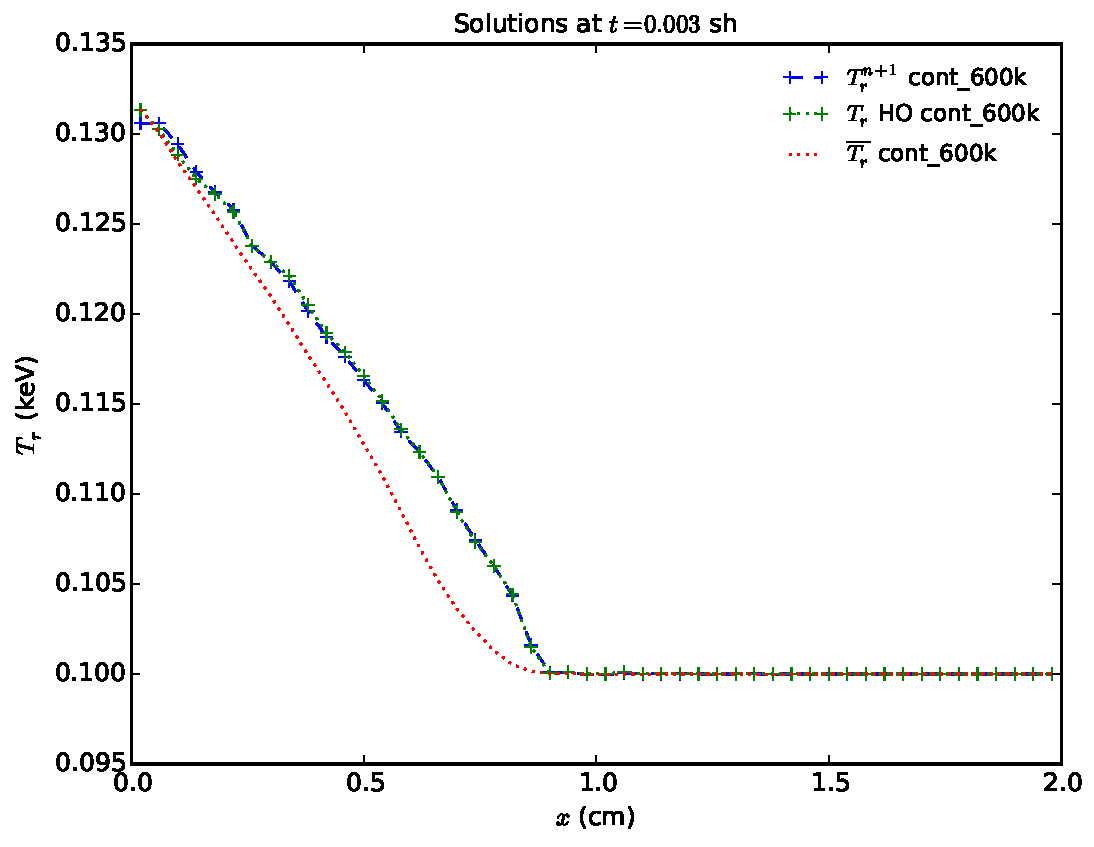
\includegraphics[width=0.65\textwidth]{void_imc_compare.pdf}
    \caption{\label{fig:void_imc_compare} Comparison of radiation energy densities of IMC
    and HOLO method for the HO time closure and a BE discretization.}
\end{figure}

A comparison of the cell-averaged radiation energy densities $E_r$ for IMC and the HOLO
method with the diamond-like HO time closure are depicted in Fig.~\ref{fig:void_imc_compare},
both for the time-averaged solutions and end-of time step values, from the final time
step.  The end of time step value for the HOLO method with a BE discretization is also depicted.
For the HOLO results, three ECMC batches were performed with
a total of $3\times10^6$ histories per time step and the IMC results were generated with
$12\times10^6$ histories per time step. 
The minimum number of histories for any sampled space-angle cell, $N_{\min}$ in
Eq.~\eqref{eq:sys_N}, is 20 for all HOLO simulations.
The spatial meshs had 100 spatial cells and both
HOLO results used 20 $\mu$ cells.  
The MC treatment of the time
variable and the closure of the LO equations allow the LO results to correctly reconstruct
the wave-front location of IMC, whereas the BE discretization artificially propagates
energy.   Although not plotted, the results were visually equivalent for either the diamond-like or implicit-like
closures in this problem.  This is because the problem is nearly linear due to the small
cross sections, so the HO moments are reproduced accurately, independent of the chosen closure
equation.  

A comparison of the same results depicted as radiation temperatures is given in Fig.~\ref{fig:void_temp_compare}.  By plotting
proportional to the fourth-root of the radiation energy density, the noise at low
magnitudes past the wave-front are more apparent in the 3 batches and $\Delta t = 0.001$
case.  This noise is small relative to the scale of $E_r$, but it demonstrates a
defficiency of the trial space.  The step representation over
the time step leads to particles sampled near the wave-front with a time near
$t^{n}$ that travel into the equilibrium region.  This is not a
bias, but rather an undersampling; if sufficient histories were performed there
would be negative particles that canceled out this error. The ECMC iterations can lead to negative
averages in the HO solution out front of the wave front.  In such cells, the
average was set to the floor value and slopes to zero. This effect is
significantly reduced when a smaller time step is taken, although the projection error is
increased.

For the case of a single batch, 
there is less noise past the wavefront because the
choice of $I^{n}(x,\mu)$ as an initial guess for $I^{n+1}(x,\mu)$ prevents most particles from
traveling past what the physical transport should allow.  The discrepancy betweeen the IMC
and the single batch HOLO solution near the foot of
the wave is a result of the spatial discrepancy between the LDFE HO projection and the
lumped LD LO equations; this dispersion is not present in the HO solution.  This
discrepancy can also lead to some negativities in the LD edge values of
$\phi^{n+1}(x)$, which are set to the floor value for the next time step. 
\begin{figure}[H]
  \centering
    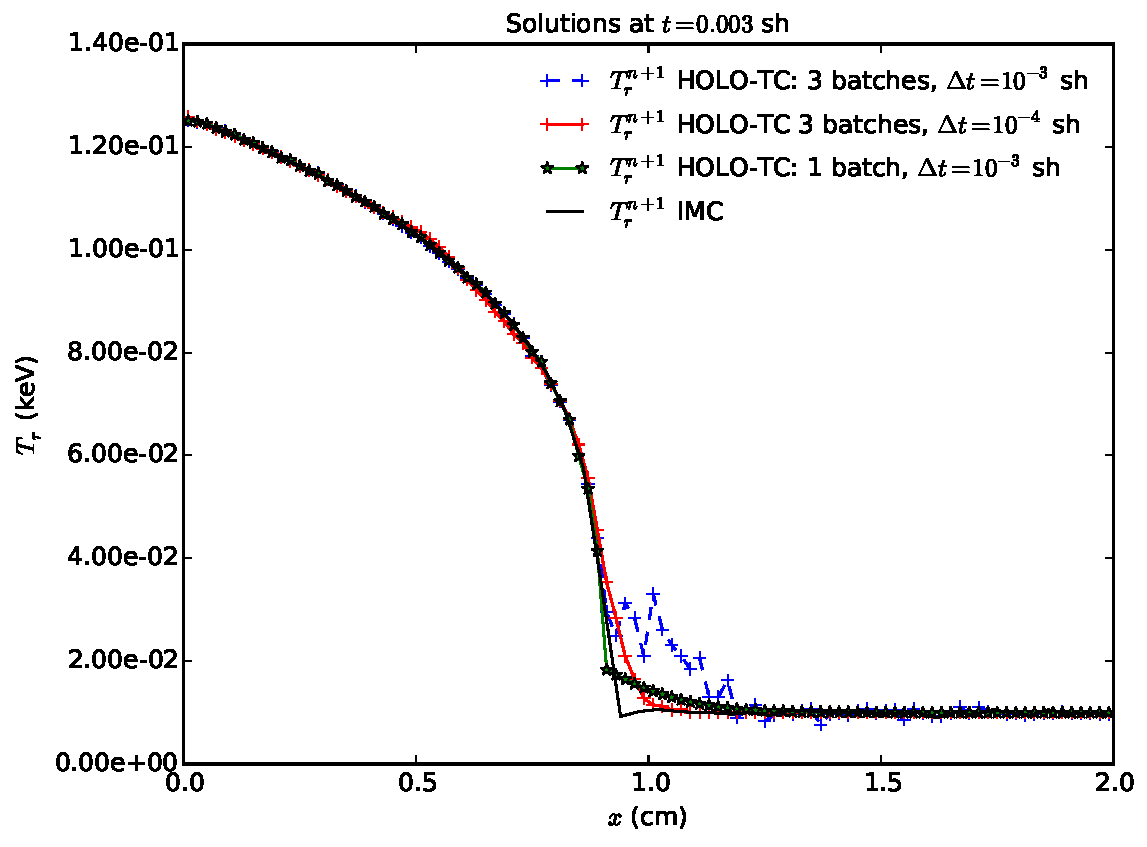
\includegraphics[width=0.75\textwidth]{void_temp_batch_compare.pdf}
    \caption{\label{fig:void_temp_compare} Comparison of radiation temperatures of IMC and
    the HOLO method for different time step sizes and numbers of batches, for the
near-void problem.}
\end{figure}

\begin{figure}[H]
  \centering
    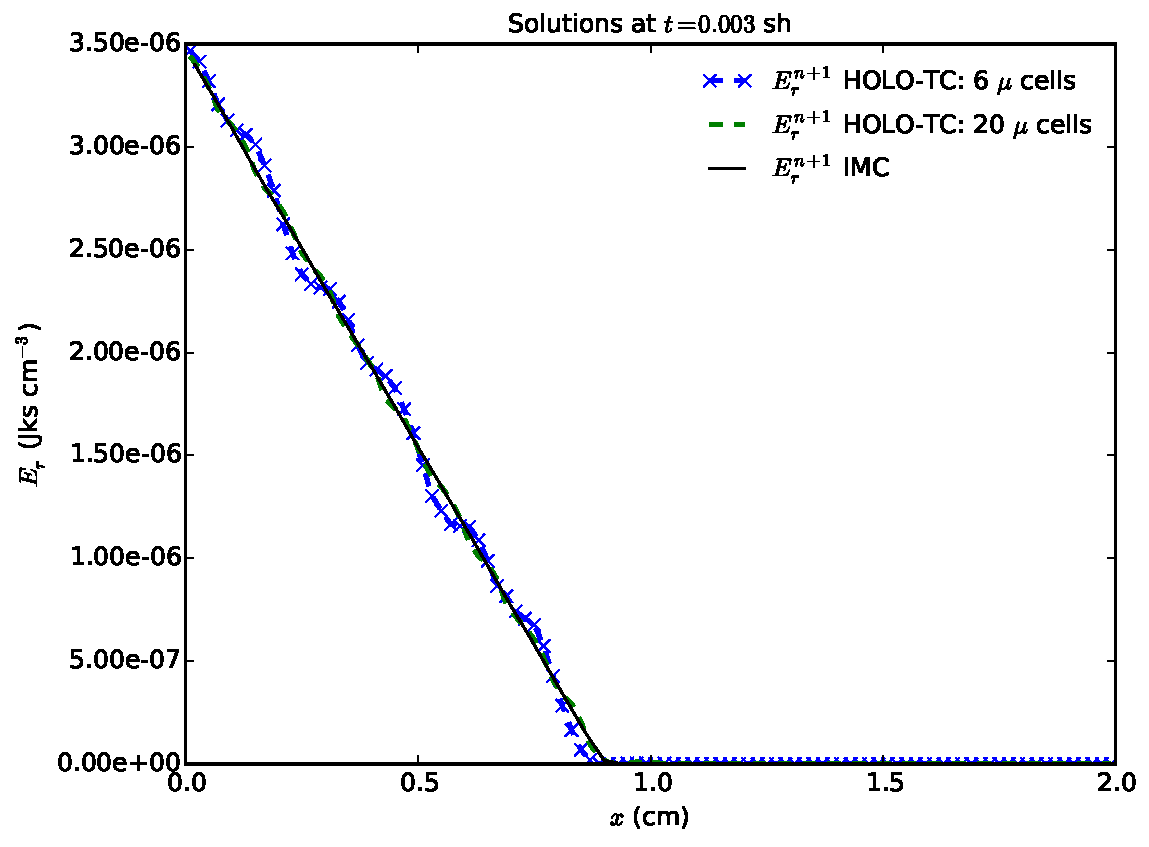
\includegraphics[width=0.75\textwidth]{void_ang_compare.pdf}
    \caption{\label{fig:bumps} Comparison of radiation energy densities for
    the HOLO method with different numbers of $\mu$ cells. $\Delta t=0.001$ sh, for
near-void problem.}
\end{figure}

Figure.~\ref{fig:bumps} compares radiation energy densities for various numbers of $\mu$
cells.  At coarser mesh sizes, the imprinting of the mesh is visible in the location of
the wave-front.  This is a result of the projection onto the space-angle mesh between time
steps.  As the mesh is refined, the solution converges towards the IMC solution.  
Smaller time step sizes can increase the mesh imprinting because the projection onto the
trial space happens more often.  However, it is important to note that this problem is a
limiting case; the mesh imprinting will be reduced as $\sigma_a$ is increased and
absorption-emission events smooth the angular intensity across each time step.

%We have computed FOM statistics using Eq.~\eqref{eq:fom} with 20 independent runs for each
%problem set up and parameters.  The statistics are computed based on the time-averaged
%radiation energy densities.  
%It is noted that the FOM results for each time step size are normalized to the IMC results within
%that table.  
%The results are compared for two different time step sizes 
%in Tables~\ref{tab:void_long} and \ref{tab:void_short}.   The different number of batches for the HOLO methods are
%indicated in parenthesis next to the method names.  The results demonstrate that IMC can
%be more efficient than the ECMC method at longer time step sizes.  This is a limiting case; because minimal absorptions are
%occuring in this problem, the IMC method is just advancing the initially sampled census particles
%between time steps, so there is negligible resampling of the phase space.  Whereas, ECMC
%must resample the residual source and the step trial-space on the interior of the tiem
%step has a larger truncation error. At smaller time step sizes,
%the ECMC method, particularly for the single batch case, becomes more efficient than IMC.
% THESE RESULTS ARE FOR THE CENSUS CASE
%\begin{table}[H]
%\centering
%\caption{\label{tab:void_long} \textbf{Comparison of sample statistics for the Near-Void
%    problem and $\Delta t = 0.001$ sh.   Simulation end time is $\mathbf{t=0.003}$ sh.}}
%\vspace{-0.1in}
%\begin{tabular}{|c|ccc|ccc|}\cline{2-7}
%    \multicolumn{1}{c|}{}       & \multicolumn{3}{|c|}{\ss} &
%    \multicolumn{3}{|c|}{\FOM} \\ \hline
%hists./step   & IMC & HOLO-TC (1) & HOLO-TC (3) &  IMC   & HOLO-TC(1) & HOLO-TC(3) \\ \hline
%   300,000    & 1.01\% & 1.39\% & 1.39\%    &       1.00  & 0.53       & 0.53       \\
%  3,000,000   & 0.32\% & 0.25\% & 0.46\%     &      0.97  & 1.68       & 0.48      \\ \hline
%\end{tabular}
%\end{table}
%
%\begin{table}[H]
%\centering
%\caption{\label{tab:void_short} \textbf{Comparison of sample statistics for the Near-Void
%    problem and $\Delta t = 10^{-4}$ sh.   Simulation end time is $\mathbf{t=0.003}$ sh.}}
%\vspace{-0.1in}
%\begin{tabular}{|c|ccc|ccc|}\cline{2-7}
%    \multicolumn{1}{c|}{}       & \multicolumn{3}{|c|}{\ss} &
%    \multicolumn{3}{|c|}{\FOM} \\ \hline
%hists./step   & IMC & HOLO-TC (1) & HOLO-TC (3) &  IMC   & HOLO-TC(1) & HOLO-TC(3) \\ \hline
%   30,000     & 3.15\%  & 0.54\% & 1.99\%       &  1.00  & 34.40      & 2.51        \\
%  300,000     & 1.01\%  & 0.13\% & 0.40\%       &  0.97  & 53.48      & 6.09        \\ \hline
%\end{tabular}
%\end{table}


%\begin{table}[H]
%\centering
%\caption{\label{tab:void_long} \textbf{Comparison of sample statistics for the
%    time-averaged radiation energy densities, of the last time step, for the near-void
%    problem and $\Delta t = 0.001$ sh.   Simulation end time is $\mathbf{t=0.003}$ sh.}}
%\vspace{-0.1in}
%\begin{tabular}{|c|ccc|ccc|}\cline{2-7}
%    \multicolumn{1}{c|}{}       & \multicolumn{3}{|c|}{\ss} &
%    \multicolumn{3}{|c|}{\FOM} \\ \hline
%hists./step   & IMC & HOLO-TC (1) & HOLO-TC (3) &  IMC   & HOLO-TC(1) & HOLO-TC(3) \\ \hline
%   300,000    & 0.27\% & 0.27\% & 0.45\%     & 1.00       &  0.96     & 0.35      \\
%  3,000,000   & 0.09\% & 0.06\% & 0.15\%     & 1.04       &  2.19     & 0.33      \\ \hline
%\end{tabular}
%\end{table}
%
%\begin{table}[H]
%\centering
%\caption{\label{tab:void_short} \textbf{Comparison of sample statistics for the
%    time-averaged radiation energy densities, of the last time step, for the near-void
%    problem and $\Delta t = 10^{-4}$ sh.   Simulation end time is $\mathbf{t=0.003}$ sh.}}
%\vspace{-0.1in}
%\begin{tabular}{|c|ccc|ccc|}\cline{2-7}
%    \multicolumn{1}{c|}{}       & \multicolumn{3}{|c|}{\ss} &
%    \multicolumn{3}{|c|}{\FOM} \\ \hline
%hists./step   & IMC & HOLO-TC (1) & HOLO-TC (3) &  IMC   & HOLO-TC(1) & HOLO-TC(3) \\ \hline
%   30,000     & 2.46\%  & 0.44\% & 1.65\%       &  1.00  & 31.07      & 2.22       \\
%  300,000     & 0.80\%  & 0.12\% & 0.37\%       &  0.95  & 43.66      & 4.47       \\ \hline
%\end{tabular}
%\end{table}



\subsection{Optically Thin Problem}

We modify the previous problem by increasing the absorption cross section to 0.2
\invcm; all other problem parameters are the same.  Radiation temperatures at the end of
the last time step are compared for IMC, HOLO-TC, and HOLO-BE in
Fig.~\ref{fig:thin_temp_compare}.  The HOLO-TC and HOLO-BE results were generated with 30
$\mu$ cells, and all spatial meshes used 100 cells.  At smaller time step sizes, the
effects of mesh imprinting are visually apparent in the HOLO-TC results, leading to more
dispersion near the wave-front.  There is good agreement between
the HOLO-TC results and IMC, except some dispersion near the wavefront.
As in the previous problem, the HOLO-BE results are very
inaccurate at capturing the wavefront location. 
IMC demonstrates substantial statistical noise in the equilibrium region.

\begin{figure}[H]
  \centering
    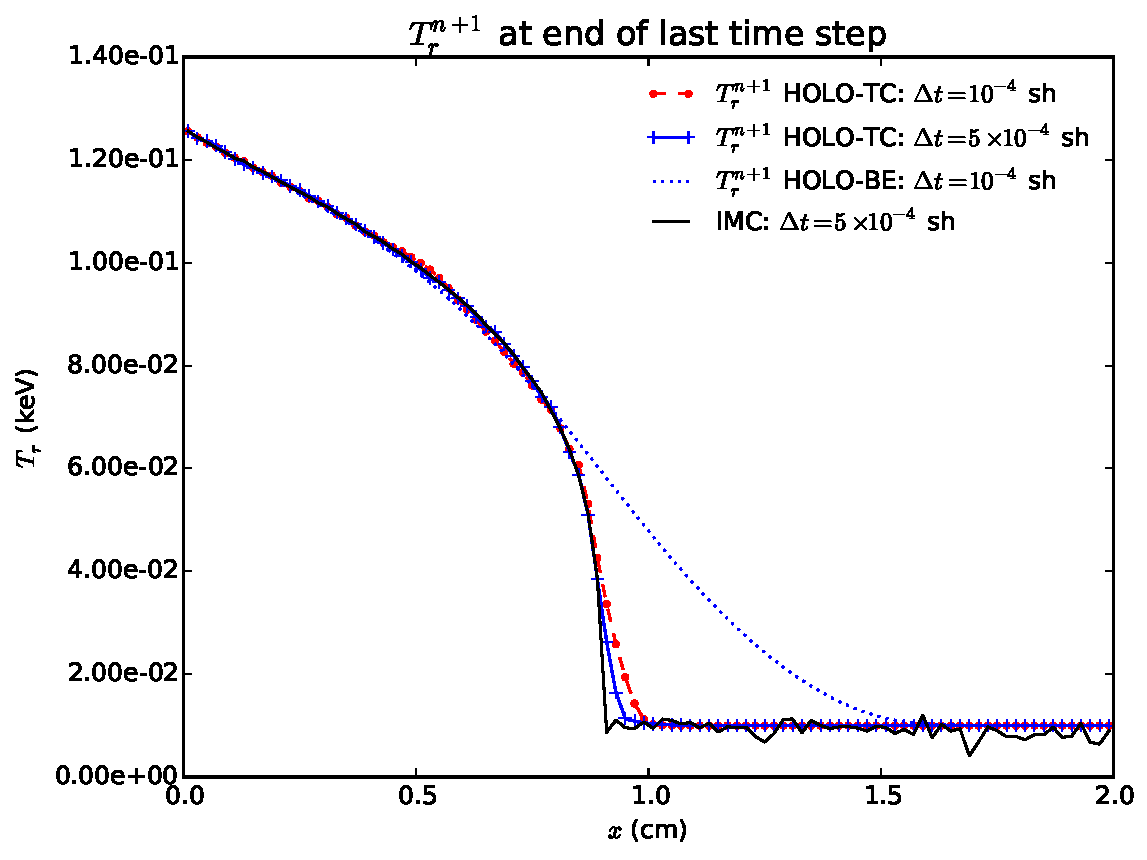
\includegraphics[width=0.75\textwidth]{thin_temp_compare.pdf}
    \caption{\label{fig:thin_temp_compare} Comparison of radiation temperatures of IMC and
    the HOLO method for different time step sizes and numbers of batches, for optically
thin problem. }
\end{figure}

The accuracy of the HOLO-TC and IMC method were compared against a reference IMC solution.
Because the material is loosely coupled in this problem we expect IMC to be accurate with sufficient particle
histories.  The
reference solution is the average of 20 IMC simulations of $20\times10^6$
histories, each with $\Delta t =10^{-4}$ sh.  The estimated value of $\ss$ for the
reference solution is 0.025\%.  The L$_2$ norm of the error in cell-averaged mean
intensities is computed using Eq.~\eqref{eq:avg_err} for $\phi^{n+1}$ from the last time
step, averaged over 20 simulations.  Sample statistics for cell-averaged $\phi^{n+1}$ were also computed using the $\FOM$
from Eq.~\eqref{eq:fom}.

Table.~\ref{tab:fom_thin} compares computed values of $\|e_a\|$ and FOM for the census
radiation energy densities, for the case of $\Delta t =
0.0005$~sh.   HOLO results were generated for the case of 1 and 2 batches, with the same
total number of histories per time step, where the number of batches is indicated in
parenthesis. The standard deviation of each estimate of $\|e\|_a$ follows each value in parenthesis. 
At low particle counts, the HOLO-TC method demonstrates substantial noise.   
A plot
of the inaccuracies for the case of 30,000 histories and a single batch is given in
Fig.~\ref{fig:30k_fails}.  As demonstrated, statistical noise in the estimate of
$\tilde I^{n+1}$ introduce instabilities into the LO result.
This is due to the trial space representation of the
census particles at the end of the time step being poorly estimated.  For the 2 batch
case, there is less error in the estimate of $\tilde I^{n+1}(x,\mu)$ because only the
deviation form the first batch estimate of $\overline I(x,\mu)$ is estimated with MC. 
At higher history counts there is an increase in efficiency, however the IMC method is
more accurate overall due to the projection error between time steps.  For reference, statistics were measured for the HOLO-BE method with two batches of 150,000
histories per time step, producing $\|e\|_a=10.5\%$ and $\FOM=3100$, demonstrating
substantial inaccuracy but improved efficiency.

Table~\ref{tab:thin_short} compares results for $\Delta t = 0.0001$~sh.  The results were
generated for two different mesh sizes, but $\|e_a\|$ is computed using the same 100
spatial cell reference solution in both cases.  All FOM values are relative to $IMC$ with
100 $x$ cells and 30,000 histories.  At the coarser mesh size, the HOLO-TC method has a
factor of 95 higher FOM, indicated much-improved statistical efficiency.  However, the projection error
limits accuracy to around 1.5$\%$.  At the finer mesh size, the
HOLO-TC method remains more efficient (as long as the batch size is sufficient) and produces higher accuracy than the IMC results.
For reference, statistics were measured for the HOLO-BE method with two batches of 150,000
histories per time step. The HOLO-BE results produced $\|e\|_a=3.7\%$ and $\FOM=4700$ for the
coarse mesh, and $\|e\|_a=3.6$ and $\FOM=9600$ for the fine mesh.  The accuracy of the HOLO-BE method
is limited by the time integration accuracy.
\begin{figure}
    \centering
    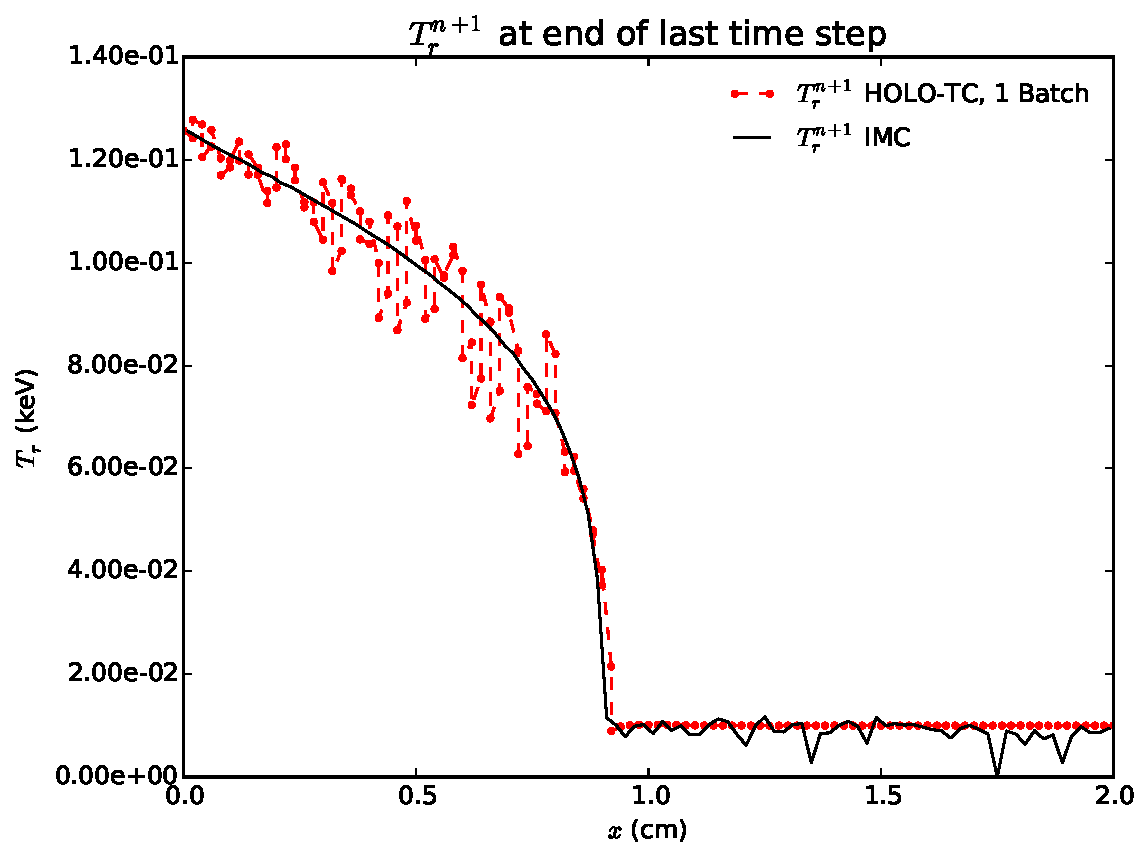
\includegraphics[width=0.75\textwidth]{thin_30k_fails.pdf}
    \caption{\label{fig:30k_fails}Comparison of $T_{r}^{n+1}$ for 30,000 histories per time step.  The HOLO-TC result has inssuficient
histories to accurately estimate end of time step unknowns.}
\end{figure}

\begin{table}[H]
\centering
\caption{\label{tab:fom_thin} {Comparison of accuracy and $\FOM$ for the
    end of time step radiation energy densities, of the last time step, for the optically
    thin problem and $\Delta t = 5\times 10^{-4}$ sh.   Simulation end time is ${t=0.003}$ sh.}}
    \resizebox{\textwidth}{!}{
\begin{tabular}{|c|ccc|ccc|}\cline{2-7}
    \multicolumn{1}{c|}{}       & \multicolumn{3}{|c|}{$\|e\|_a$} &
    \multicolumn{3}{|c|}{\FOM} \\ \hline
hists./step   & IMC & HOLO-TC (1) & HOLO-TC (2)    &  IMC   & HOLO-TC(1) & HOLO-TC(2) \\ \hline
   30,000     & 3.0\% $(0.08\%)$   & 17.3\% $(0.5\%) $  & 4.99\%  $(0.2\%) $    &  1.00  & 0.03  &  0.31      \\
  300,000     & 1.0\% $(0.02\%)$   & 1.1\%  $(0.02\%)$  & 1.13\%  $( 0.02\%)$    &  0.93  & 1.38  &  1.65     \\ 
  1,000,000   & 0.5\% $(0.01\%)$   & 0.92\% $(0.01\%)$  & 0.96\%  $(0.01\%)$    &  1.10  & 3.42  &  2.0      \\ \hline
\end{tabular}
}
\end{table}

\begin{table}[H]
\centering
\caption{\label{tab:thin_short} {Comparison of accuracy and $\FOM$ for the end of time
    step radiation energy densities, of the last time step, for the optically
    thin problem and $\Delta t = 1\times 10^{-4}$ sh.  The reference results are all for 100 $x$ cells.
    Simulation end time is ${t=0.003}$ sh.}}
\vspace{-0.1in}
\begin{tabular}{|c|cc|cc|}\cline{2-5}
    \multicolumn{1}{c|}{}       & \multicolumn{2}{|c|}{$\mathbf{\ss}$} &
    \multicolumn{2}{|c|}{\textbf{\FOM}} \\ \hline
hists./step   & IMC     & HOLO-TC (1) &    IMC   & HOLO-TC(1)  \\ \hline
\multicolumn{5}{|c|}{Results for 100 $x$ cells; HOLO-TC has 30 $\mu$ cells} \\ \hline
   30,000     & 2.98\% $(0.09\%)$   & 1.49\% $(0.02\%)$          &  1.00  &  42.0      \\
  300,000     & 0.96\% $(0.02\%)$   & 1.45\% $(<0.01\%)$         &  0.98  &  94.5      \\ 
  1,000,000   & 0.49\% $(0.01\%)$  & 1.45\% $(<0.01\%)$         &  1.11  &  94.9      \\ \hline
\multicolumn{5}{|c|}{Results for 200 $x$ cells; HOLO-TC has 60 $\mu$ cells} \\ \hline
   30,000     & 2.93\% $(0.1\%)$   & 14.00\% $(0.4\%)$    & 0.49   &  0.05      \\
  300,000     & 0.99\% $(0.03\%)$  & 0.37\% $(<0.01\%)$   & 0.45   &  6.98      \\ 
  1,000,000   & 0.49\% $(0.01\%)$  & 0.18\% $(<0.01\%)$   & 0.50   &  40.04      \\ \hline
\end{tabular}
\end{table}

\subsection{Marshak Wave Problem}

It is important to demonstrate that the time closures are stable in a mix of optically
thick and optically thin regions, and that the ECMC method is still efficient in such
problems.  Simulations were performed for the Marshak wave problem defined in
Sec.~\ref{sec:marsh}.  The time step size is linearly increased from $0.001$ sh to a
maximum step of 0.01 sh over the first 10 time steps; the last time step is adjusted to
reach the desired simulation end time.  It was found for this problem that it was
necessary to use more than one batch for the HOLO-TC algorithm to stably converge, for the
same reasons inaccuracies were demonstrated in the previous section.  
\begin{figure}[H]
    \centering
    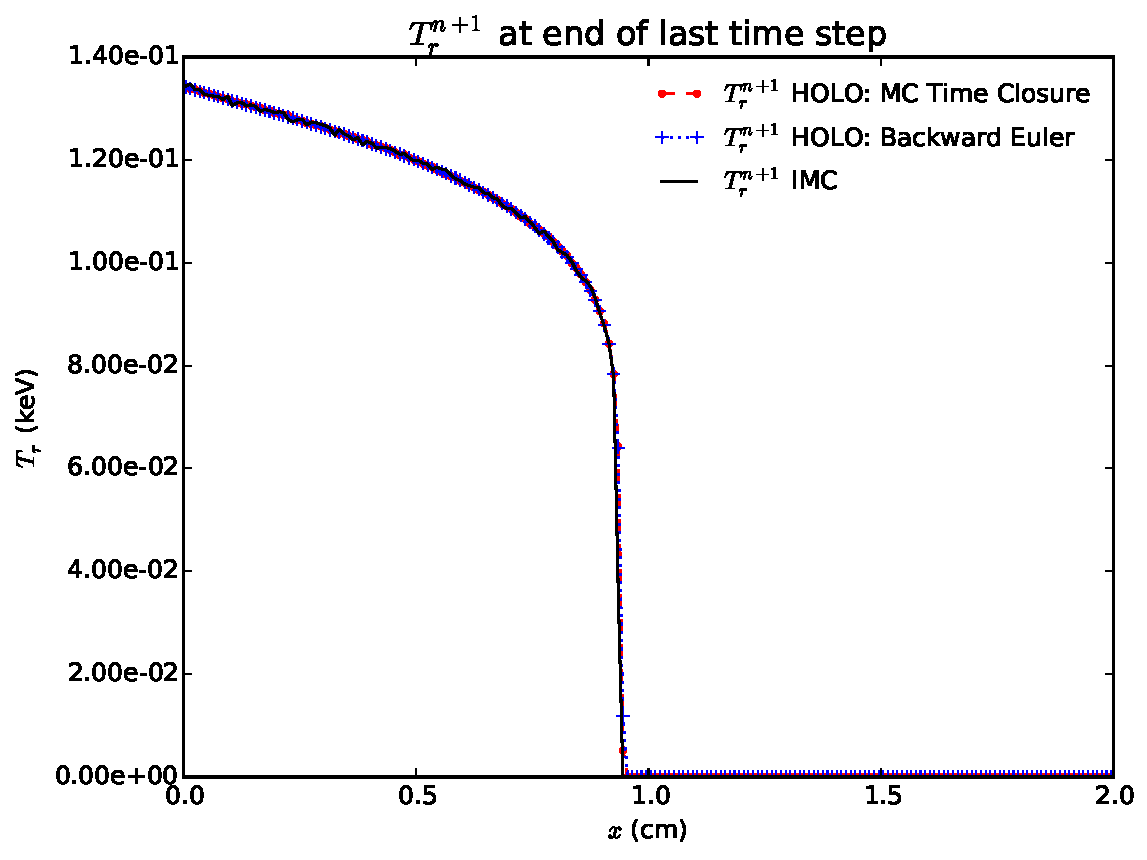
\includegraphics[width=0.65\textwidth]{marshak_time_cont_compare.pdf}
    \caption{\label{fig:marshak_tc} Comparison of HOLO-TC, HOLO-BE, and IMC methods for
the Marshak Wave problem, with $10^6$ histories per time step.}
\end{figure}

Figure~\ref{fig:marshak_tc} compares the accuracy of IMC, HOLO-TC, and HOLO-BE. 
These results were generated using the implicit-like time
closure. The
solutions are plotted at $t=3$ sh, with $10^6$ histories per time step for all
simulations. As demonstrated, there is good agreement among the results.  It is noted that
this problem can be accurately modeled with the Backward Euler time discretization, but
the MC time closure appears to be stable even in the mix of optically thick and thin
regions. Table~\ref{tab:marshak_cont} compares sample statistics for IMC,
the HOLO-TC method with the implicit-like and diamond-like closures, and the HOLO-BE
method.  As demonstrated, at the lower history count (300,000), the HOLO-TC algorithm demostrates a
greater variance than IMC, but is more efficient at the higher batch size.  The HOLO-BE
method is signficantly more efficient for comparable accuracy in this problem with a very
optically thick region.
\begin{table}[H]
\centering
\caption{\label{tab:marshak_cont} {Comparison of sample statistics for the
    end of time step radiation energy densities, of the last time step, for the marshak
    wave problem and maximum time step of $0.01$ sh.  Simulation end time is $\mathbf{t=3.0}$ sh.}}
\vspace{-0.1in}
\begin{tabular}{|c|ccc|ccc|}\cline{2-7}
    \multicolumn{1}{c|}{}       & \multicolumn{3}{|c|}{\ss} &
    \multicolumn{3}{|c|}{\FOM} \\ \hline
hists./step   & IMC & HOLO-TC (2) & HOLO-BE (2) &  IMC   & HOLO-TC (2) & HOLO-BE (2) \\ \hline
  \multicolumn{7}{|c|}{HOLO-TC using Implicit-Like Closure} \\ \hline
  300,000     & 2.25\%  & 3.42\% & 0.30\%       &  1.00  &   0.43    & 2050          \\  
  1,000,000   & 1.27\%  & 0.31\% & 0.17\%       &  0.94  &  15.95    & 1806          \\ \hline
  \multicolumn{7}{|c|}{HOLO-TC using Diamond-Like Closure} \\ \hline
  300,000     & --  & 3.53\% & --   &  --  &   0.41   & --  \\  
  1,000,000   & --  & 0.37\% & --   &  --  &  10.94   & --  \\ \hline
\end{tabular}
\end{table}

\subsubsection{Importance Sampling on Interior of the Time Step}

The importance sampling algorithm
detailed in Sec.~\ref{sec:imp_sampling} was investigated for the Marshak wave problem.  In
particular, various values of $p_{surv}$ with a fixed value of 2 MFP of survival distance
were investigated.  Sample statistics were measured for the HOLO-TC algorithm and the case of two batches of
100,000 histories per time step, with a max time step size of 0.01 sh.    The importance
sampling algorithm was found to generally increase the variance for this problem.  This
is likely caused by the fact that when no importance sampling is used, in the very thick
cells essentially no particles reach the census.  In such cells, because the ECMC
algorithm is estimating the difference between the first batch's estimate of
$\overline{I}(x,\mu)$ and $\tilde I^{n+1}(x,\mu)$, it just accepts $\overline I(x,\mu)$ as
$I^{n+1}(x,\mu)$.  The initialization of the solution to the first batches estimate of
$\overline{I}(x,\mu)$ is sufficient to produce visually accurate results because the
problem is evolving slowly, although this a biased result due to undersampling
of the phase space. When importance sampling is used, then more particles reach
the census, increasing variance overall.  If too many particles are sampled near the end
of the time step, then the variance of the time-averaged solution
increases, decreasing accuracy over all. 
\begin{table}[H]
\centering
\caption{\label{tab:void_short} {Comparison of sample statistics using importance
    sampling on the interior of the time step, for the Marshak Wave problem.  Simulation
    end time is $\mathbf{t=1.0}$ sh.} and max $\Delta t$ is 0.01 sh}
\vspace{-0.1in}
\begin{tabular}{|cc|} \hline
        $p_{surv}$ & {\FOM} \\ \hline
       No Bias & 1 \\ 
       0.05    & 0.001 \\
       0.1     & 0.005 \\
       0.25    & 0.179  \\
       0.5     & 0.003 \\ \hline
\end{tabular}
\end{table}









